\section{Data}
\label{sec:data}

\subsection{Capture: the smart cube is a label, never an input}
\label{sec:capture}

Each recording session runs two devices on one wall clock: a webcam at
30\,fps writing JPEG frames with timestamps, and a GoCube-protocol Bluetooth
cube streaming move events. The cube's move stream is written to
\file{moves.jsonl} and is used \emph{only} as supervision and as evaluation
ground truth. It is never an input to any model, and no inference path reads
it. This is the single most important discipline in the data pipeline,
because the whole point of the product is a claim decided from video alone;
a model that had ever seen the BLE stream at inference would be measuring
nothing.

\begin{keybox}
\textbf{Why this is a good deal.} Dense temporal supervision for video is
normally the expensive part. Here it is free and exact: \NMovesTotal\
labelled turns across \NSessionsFrames\ sessions, with no human annotation. That is what made a
supervised approach viable for one person over three weeks. It is also the
project's biggest strategic weakness, because it ties the training corpus to
people who own a specific piece of hardware --- \cref{sec:gap} returns to
this.
\end{keybox}

Two artefacts of the BLE channel matter numerically.

\paragraph{Timestamp collisions.} The cube's event tick is 30\,ms and the
camera runs at 30\,fps, so turns performed in quick succession are not
separable in time. Measured over the whole corpus (\CorpusOnsets\ turns):
\CorpusCrowdedTwo\% of turns land within two frames of a neighbour,
\CorpusCrowdedOne\% within one, and \CorpusSameFrame\% on the
\emph{same} frame. That last group is the hard one --- for an
alignment-supervised model the labels literally ask for two peaks in one
frame, which no model can satisfy. For CTC it costs nothing, because CTC is
supervised on order only. This is one of the two reasons the project
migrated to CTC.

(The repository quotes ``10.1\% of moves collide''. That is the
within-two-frames figure, which is not the same as the unassignable set and
is roughly $8\times$ larger; the distinction matters when deciding what a
different objective would actually buy.)

\paragraph{The end-state query is unreliable.} The cube's ``what state are
you in'' query returns a constant 36-facelets-wrong answer on solved cubes
in this firmware. The move \emph{event} stream is fine --- composing a
session's own move word from its start state reaches solved --- so all
ground truth here is derived from the move log, never from the state query.

\subsection{Preprocessing}
\label{sec:preproc}

\begin{enumerate}[leftmargin=1.4em,itemsep=3pt]
\item \textbf{Locate the cube.} A fine-tuned YOLOv8n detector runs every
10th frame. Its boxes are median-smoothed over time and then linearly
interpolated to every frame. Interpolating rather than detecting per frame
is deliberate and non-obvious: the detector's frame-to-frame box jitter,
once used as a crop, injects apparent global motion into the very temporal
difference the model reads as its onset signal. Smoothing removes a
distractor that is correlated with nothing.
\item \textbf{Crop and resize} to $96\times96$, keeping BGR.
\item \textbf{Build four channels}: the three colour channels, each centred
to $[-\tfrac12,\tfrac12]$, plus a signed luma difference
$\Delta_t = \mathrm{luma}(f_t) - \mathrm{luma}(f_{t-1})$.
\end{enumerate}

\Cref{fig:input} shows all four channels on real held-out frames. The
difference channel is where the turn is legible: a layer rotation produces a
structured, spatially-localised difference pattern, whereas a regrip or a
whole-cube rotation produces a \emph{larger} but globally coherent one. That
distinction is exactly what a magnitude threshold cannot make and a learned
appearance model can, and it is the second reason the peak-picking arm was
abandoned.

\begin{figure}[t]
\centering
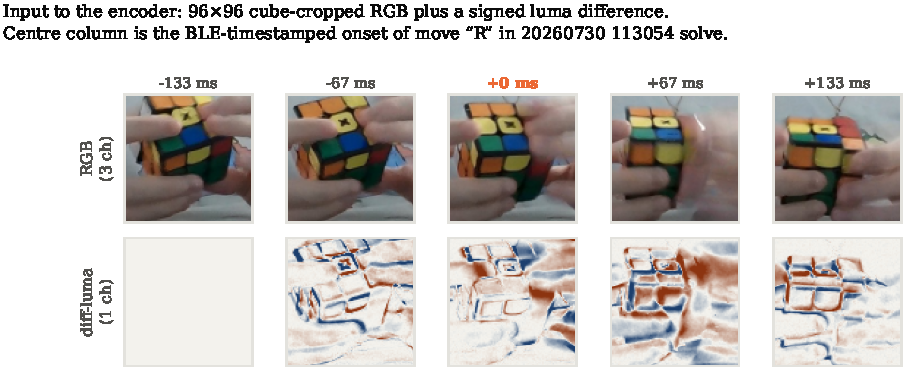
\includegraphics[width=\linewidth]{figures/fig_input.pdf}
\caption{The encoder's input on five consecutive held-out frames spanning
one ground-truth turn. Top: the cube-cropped colour channels. Bottom: the
signed luma difference (blue negative, orange positive). The first
difference panel is flat because the cube was genuinely still 133\,ms before
the turn --- that is the signal, not a rendering artefact. Note that the
turn is visible in the difference channel two frames \emph{before} the BLE
timestamp, which is the ${\sim}1$-frame label jitter discussed in
\cref{sec:labelnoise}.}
\label{fig:input}
\end{figure}

\paragraph{Crop-regime provenance.} The crop mode used to build each stream
is recorded inside the stream file and checked at train, eval and inference
time. This guard exists because of a real and expensive failure: for a
period the trainer silently fell back to \emph{uncropped} full frames for
sessions that lacked a cached crop, while inference always cropped. The
resulting evaluation compared a full-frame-trained model against
cropped-input test data and reported a 61.5\% aggregate that was really
90.6\% once the evaluation was made consistent. Nothing about the models had
changed. The lesson generalises past this project: \emph{when a retrain
appears to fix a regime, check what else changed about the data before
crediting the fix to the thing you meant to change.}

\subsection{The label frame problem}
\label{sec:labelframe}

The smart cube names turns relative to its own core. A middle-slice turn
(\wca{M}, \wca{E}, \wca{S}) --- which speedcubers perform constantly, and
which the cube reports as a pair of outer-layer turns --- rotates that core.
From that moment the cube's frame has rotated away from the camera's, and
every subsequent label names the wrong face. Two slices (\wca{M2}, common in
last-layer algorithms) and the cube calls the physically-top face \wca{D}
while the camera correctly sees \wca{U}.

This hid for a long time for an instructive reason. The repository's
session-consistency check applies each label to a \emph{cubie} model, which
has no centres and is therefore centre-relative by construction. It
validates the cube-frame product and is structurally blind to camera-frame
drift. It reported 16/16 sessions consistent throughout.

\begin{keybox}
\textbf{Never read a passing endpoint check as evidence about the frame of
reference.} A check that composes labels into a group element cannot see a
relabelling that composes to the identity, and the drift here \emph{does}
cancel: every affected session returns to identity by the end.
\end{keybox}

Scope: \SliceSessions\ sessions in the corpus contain slices, and because the drift
cancels, only \SliceMoves\ moves corpus-wide are actually misnamed
($\SliceMovePct$\%). It is a correctness fix, not an accuracy lever. But it
is still live in the repository: \emph{every} evaluation harness in
\file{ble/move\_detector/} scores against the cube-frame name, while
\file{prepare\_data.py} has trained against the camera-frame name since
2026-08-03. All measurements in this report use the camera frame.
\cref{sec:frame-result} quantifies the difference: on the three
slice-bearing held-out sessions it is worth $\FrameGainSlice$ points, and
$\FrameGainAll$ points averaged over the whole holdout.

\subsection{Label noise}
\label{sec:labelnoise}

Even without slices the labels are not exact. Aligning BLE timestamps to
frame timestamps gives a median offset of 6--10\,ms with a maximum around
33\,ms, i.e.\ up to one frame. This is irreducible at 30\,fps and is one
reason an order-only objective (CTC) is a better fit than an alignment
objective: CTC's loss is invariant to it, whereas Gaussian-target
supervision is asked to place a peak on the wrong frame roughly half the
time.

\subsection{Corpus and holdout policy}
\label{sec:holdout-hygiene}

The corpus is \NSessionsFrames\ sessions with usable frames across
\NDays\ distinct days, \NMovesTotal\ labelled turns, one solver, one cube,
two rooms. Sessions come in pairs: a \emph{scramble} take (a
machine-generated ${\sim}20$-move sequence performed slowly from a printed
prompt --- every move known exactly) and a \emph{solve} take (a free solve;
long, fast, and the regime that matters).

\paragraph{The holdout rule used here.} A session is evaluable for a
checkpoint if and only if its name appears in neither that checkpoint's
recorded \texttt{train\_session\_names} nor its
\texttt{val\_session\_names}. When several checkpoints are compared, the
holdout is the \emph{intersection} across all of them. This is computed from
the checkpoint files themselves, not from a maintained list.

Validation sessions are excluded on purpose. They chose the stopping epoch,
so they are model-selection data; in this corpus they are also same-day
neighbours of training sessions, which makes them the most flattering
sessions available. \cref{sec:ladder} measures exactly how flattering.

\paragraph{Where this differs from the repository's own numbers.} The
repository quotes results on ``the 8 never-trained \texttt{*\_solve}
sessions''. Two of those eight are the checkpoints' validation sessions.
Under this report's rule the equivalent set is \NHoldoutSolves\ solves ---
larger, because I prepared \NewlyPrepared\ sessions that had been recorded
but never run through preprocessing, and therefore had never been evaluated
by anything.

\begin{table}[t]
\centering\small
\caption{The evaluation set. Every session listed is absent from both the
training and validation lists of every checkpoint scored in this report.}
\label{tab:holdout}
\begin{tabular}{@{}llrrrrl@{}}
\toprule
session & clock & frames & turns & turns/s & crowded & regime \\
\midrule
07-29\,22:18 scramble & 22h & 803 & 20 & 0.79 & 0\% & evening \\
07-29\,22:18 solve & 22h & 1566 & 152 & 3.08 & 23\% & evening \\
07-30\,11:19 scramble & 11h & 880 & 20 & 0.79 & 0\% & daytime \\
07-30\,11:19 solve & 11h & 1464 & 106 & 2.23 & 10\% & daytime \\
07-30\,11:30 scramble & 11h & 964 & 20 & 0.65 & 0\% & daytime \\
07-30\,11:30 solve & 11h & 1545 & 132 & 2.72 & 16\% & daytime \\
07-31\,21:10 scramble & 21h & 863 & 20 & 0.76 & 0\% & evening \\
07-31\,21:10 solve & 21h & 1123 & 84 & 2.55 & 24\% & evening \\
07-31\,21:35 scramble & 21h & 1048 & 20 & 0.59 & 0\% & evening \\
07-31\,21:35 solve & 21h & 1215 & 108 & 2.88 & 19\% & evening \\
08-03\,09:51 scramble & 09h & 1012 & 22 & 0.67 & 0\% & daytime \\
08-03\,09:51 solve & 09h & 1062 & 82 & 2.58 & 17\% & daytime \\
08-03\,09:55 scramble & 09h & 993 & 20 & 0.68 & 0\% & daytime \\
08-03\,09:55 solve & 09h & 1849 & 140 & 2.38 & 14\% & daytime \\
08-03\,10:01 scramble & 10h & 767 & 20 & 0.90 & 0\% & daytime \\
08-03\,10:01 solve & 10h & 1458 & 123 & 2.93 & 24\% & daytime \\
08-03\,12:29 scramble & 12h & 1146 & 22 & 0.67 & 0\% & daytime \\
08-03\,12:29 solve & 12h & 1345 & 120 & 2.86 & 17\% & daytime \\
08-03\,12:34 scramble & 12h & 1028 & 22 & 0.66 & 0\% & daytime \\
08-03\,12:34 solve & 12h & 1015 & 88 & 2.81 & 17\% & daytime \\
08-04\,21:42 scramble & 21h & 940 & 20 & 0.67 & 0\% & evening \\
08-04\,21:42 solve & 21h & 1625 & 116 & 2.21 & 15\% & evening \\
08-04\,23:49 scramble & 23h & 857 & 20 & 0.74 & 0\% & evening \\
08-04\,23:49 solve & 23h & 1205 & 92 & 2.42 & 19\% & evening \\
08-05\,15:58 scramble & 15h & 943 & 20 & 0.66 & 0\% & daytime \\
08-05\,15:58 solve & 15h & 1512 & 124 & 2.70 & 17\% & daytime \\
08-09\,15:57 scramble & 15h & 803 & 20 & 0.81 & 0\% & daytime \\
08-09\,15:57 solve & 15h & 884 & 88 & 3.54 & 18\% & daytime \\
\bottomrule
\end{tabular}

\end{table}

\paragraph{The corpus is drifting, and that is measurable.} The solver got
roughly twice as fast over the three weeks of recording
(\cref{fig:drift}). The fraction of adjacent turn pairs within two frames
rose from under 1\% to \CrowdedPctHoldout\% in the held-out set. The
training corpus is therefore not merely small, it is weighted toward a
regime the solver has left. This confounds any attempt to read the
day-distance effect in \cref{sec:ladder} as pure generalisation: the more
distant sessions are also the faster ones.

\begin{figure}[t]
\centering
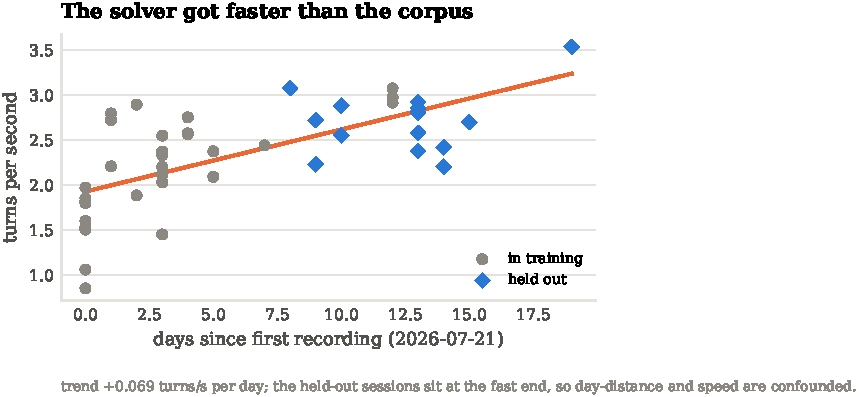
\includegraphics[width=0.86\linewidth]{figures/fig_drift.pdf}
\caption{Turn rate against recording date, every session with more than 40
turns. The held-out sessions are not a random sample of the corpus --- they
are systematically at the fast end, because they are the later ones. Any
claim of the form ``held-out accuracy is lower because the model does not
generalise across days'' is confounded with ``held-out accuracy is lower
because those solves are faster''.}
\label{fig:drift}
\end{figure}
